%!TEX root = flock-comment-main.tex

\section*{Introduction}
Methods for the unsupervised clustering of genotypes have received 
considerable attention in the molecular ecology literature.  
The best known of this class of methods is {\sc structure} 
\citep{Pritchardetal2000}, with over 12,000 citations identified on 
Google Scholar.  A variety of other 
clustering methods have been developed that are all closely related to 
{\sc structure}, for example {\sc NewHybrids} \citep{And&Tho2002}, {\sc 
BayesAss+} \citep{Wil&Ran2003}, and {\sc baps} 
\citep{Coranderetal2004}. An overview of the similarities between several of these methods can be 
found in \citet{Anderson2009PGAC}.

The recently introduced software {\sc flock} \citep{Duc&Tur2009} has
been described
as a ``non-Bayesian method [that] 
differs substantially from previous 
clustering algorithms'' \citep[][p.~1333]{Duc&Tur2009}. As reported
in a later paper, ``{\sc flock} is very different from  other clustering 
programs. It does not sample the space of partitions through small 
random step walks as in MCMC, and it does not try to optimize some 
target function, such as HWLE\@. Briefly stated, it is not based on a 
probabilistic search algorithm. On the contrary, {\sc flock} is 
entirely deterministic'' \citep[][p.~736]{Duc&Tur2012}.

Given the above sort of emphasis on the distinctiveness of the {\sc flock}
algorithm, it would not be surprising if most readers incorrectly believed {\sc flock}
to be based upon a completely different model than the well-known program
{\sc structure}. Here we remedy such confusion with a simple derivation
that identifies 
the close relationship between the {\sc flock} algorithm and the program
{\sc structure}.  Although the algorithm in {\sc flock}
is, as the authors point out, deterministic (apart from a random initial allocation of 
individuals to clusters), it can be interpreted as a 
limiting case of a probabilistic search algorithm applied to one of {\sc structure}'s
models.  More specifically, the {\sc flock} 
algorithm is a special case of the simulated annealing
algorithm for finding the Bayesian maximum-{\em a-posteriori}
estimate from a marginalized form of the {\sc structure} model with no
admixture and non-correlated allele frequencies.  Thus, while the models underlying
{\sc structure} and {\sc flock} are nearly indistinguishable, {\sc structure}'s inference
relies on MCMC samples from the posterior distribution, while
{\sc flock}'s inference involves finding local maxima in the posterior surface.

Recognizing {\sc flock}'s underpinnings in this fashion should help users
interpret output from {\sc flock} and predict when it might and might not
give substantially different results than {\sc structure}. Below we describe
the correspondence between the programs in more detail, and then, for illustration,
and to aid in application to simualted data, we
create the progam {\sc flockture} by adapting the code of {\sc structure} to 
use a simulated annealing approach. We then compare results of the two
programs from large 
data sets simulated with varying degrees of population differentiation. 

\section*{Comparison of methods}
We start with a succinct mathematical description of the {\sc structure}
model, then describe the {\sc flock} algorithm, and finally explain
the close relationship between the two.


\subsection*{{\sc structure}}
In the {\sc structure} model with no admixture (which, it should be pointed out, 
is not the default model in {\sc structure}), the unknown ``subpopulation'' that the 
$i\thh$ individual ($i=1,\ldots,N)$ belongs to is denoted by $Z_i \in \{1,\ldots,K\}$, 
where $K$ is the 
number of subpopulations (or clusters, as they are often referred to).  
In a diploid individual from cluster $k$, the 
allelic types of the two gene copies at the $\ell\thh$ locus are assumed
to be drawn independently from the vector of allele frequencies at
locus $\ell$ in subpopulation $k$,  $\theta_{k\ell}=(\theta_{k\ell 1},\ldots,\theta_{k\ell A_\ell})$, where 
$A_\ell$ 
denotes the number of alleles observed in the data set at locus $\ell$.
Hence, if $Y_{i\ell}$ denotes a vector of length $A_\ell$ whose components denote the 
number
of copies of each of the $A_\ell$ alleles at locus $\ell$ in a diploid individual $i$, and 
$Z_i=k$, then $Y_{i\ell}$ follows the multinomial distribution of two trials with
$A_\ell$  components and cell probabilities given by the allele frequencies: 
\begin{equation}
(Y_{i\ell}~|~Z_i=k) \sim \mathrm{Mult}_{A_\ell}(2, \theta_{k\ell}).
\end{equation}
In the {\sc structure} model without physical linkage, the genotypes at the loci are assumed to
be independent of one another, so the probability of the genotype data at
all $L$ loci---$Y_i=(Y_{i1},\ldots,Y_{iL})$---is simply a product of multinomial 
probabilities.
In the uncorrelated allele frequencies model, the prior on each $\theta_{k\ell}$ is a
Dirichlet distribution with parameters $(\lambda_{k\ell1},\ldots,\lambda_{k\ell A_
\ell})$,
which are usually all set to a value such as 1 or $1/A_\ell$.  

After initializing the unknown allele frequencies, $\theta = (\theta_1,\ldots,\theta_K)$, to randomly drawn values from the prior,
$\theta^{(0)}$, inference in the model proceeds by sampling from the joint posterior of the 
$Z_i$'s and $\theta$ using Gibbs sampling.  That is, if Gibbs sampling is run for $T$ iterations,
at iteration $t =0, 1, 2, \ldots, T-1$:
\begin{itemize}
\item each $Z^{(t)}_i$ is updated to $Z^{(t+1)}_i$ by sampling a value from 
the full conditional distribution of $Z_i$ given
$Y_i$ and $\theta^{(t)}$ (the current estimate of the allele frequencies).  This
distribution is found using Bayes' theorem. In {\sc structure}'s formulation, the 
prior probability that $Z_i=k$ is $1/K$ for all $k=1,\ldots, K$, implying the belief that the subpopulations are equally
represented in the sample before observing the genotypes present.    
\item $\theta^{(t)}$ is updated to $\theta^{(t+1)}$ from its full conditional distribution.  For each 
cluster
$k$ and locus $\ell$, the full conditional for $\theta_{k\ell}$ is independently a 
Dirichlet distribution with parameters $\lambda_{k\ell j} + \#(k,\ell,j)$, for 
$j=1,\ldots, A_\ell$,
where $\#(k,\ell,j)$ is the number of alleles of type $j$ at locus $\ell$ observed in 
individuals with $Z^{(t+1)}_i = k$.   
\end{itemize}

It will be useful for our comparison with {\sc flock} to point out that another way 
of pursuing inference in this model would be to first integrate out the 
Dirichlet priors on the allele frequencies and then sample from the posterior
for the $Z_i$'s by Gibbs sampling.  When $\theta$ is integrated out, the genotypes 
of the individuals are no longer conditionally independent (they were originally
independent {\em conditional} on $\theta$ and the $Z_i$'s), so the calculation of 
the full conditional distribution of $Z_i$ becomes somewhat more involved,
but can be computed by the following reasoning. First, the 
conditional distribution of $Y_{i\ell}$, given that individual $i$ is from subpopulation $k$
(\ie $Z_i=k$), depends on the 
cluster memberships and genotypes at locus $\ell$ of all the remaining individuals,
which we denote by  $Z_{(-i)}$ and $Y_{(-i)\ell}$, respectively.
This full conditional for $Y_{i\ell}$ follows 
a Compound Dirichlet Multinomial distribution (CDM):
\begin{eqnarray}
\lefteqn{(Y_{i\ell}~|~Z_i=k,~Z_{(-i)},~Y_{(-i)\ell}) \sim} \label{eq:cdm}\\
& & \mathrm{CDM}(\lambda_{k\ell 1} + \#_{(-i)}(k,\ell,1), \ldots,
\lambda_{k\ell A_\ell} + \#_{(-i)}(k,\ell,A_\ell)), \nonumber
\end{eqnarray}
where $\#_{(-i)}(k,\ell,j)$ is the number of alleles of type $j$ at locus $\ell$
found in individuals {\em other than individual $i$} that currently
belong to cluster $k$. Thus, calculating the product of (\ref{eq:cdm}) across all the loci
($\ell = 1,\ldots,L$) gives the full conditional multilocus genotype probability 
for individual $i$:
\begin{eqnarray}
\lefteqn{P(Y_{i}~|~Z_i=k,~Z_{(-i)},~Y_{(-i)}) =}  \label{eq:cdm-multi-prob} \\
& &  \prod_{\ell=1}^L P(Y_{i\ell}~|~Z_i=k,~Z_{(-i)},~Y_{(-i)\ell}). \nonumber
\end{eqnarray}
Computing (\ref{eq:cdm-multi-prob}) for 
for each value of $Z_i=k \in 
\{1,\ldots,K\}$ 
and normalizing to sum to one gives the full conditional distribution for 
$Z_i$:
\begin{equation}
P(Z_i=k~|~Y_i, ~Z_{(-i)},~Y_{(-i)})~~,~~k=1,\ldots,K.
\label{eq:fc}
\end{equation}
A new value of $Z_i$ would be drawn from (\ref{eq:fc}) if doing Gibbs sampling in this
version of the {\sc structure} model in which $\theta$ has been integrated out.  In 
fact,
this is the approach (with a slightly different prior weight on the $Z_i$'s) taken to 
update 
$Z_i$ in both {\sc hwler} \citep{Pel&Mas2006} and {\sc structurama} \citep{Hue&And2007} 
when not
proposing changes to the number of clusters.



\subsection*{{\sc flock}}
Here we translate the procedure given by \citet{Duc&Tur2009} for the 
{\sc flock} algorithm into a specification in terms of the variables
defined in the previous section.  We provide the description for a case in which
it is assumed there are $K$ clusters.

The first step of the {\sc flock} algorithm is initialization, during which 
the program randomly allocates or partitions the $N$ individuals into
approximately equal-sized
clusters.  Then a number of reallocation steps are performed.  During every one of 
these steps, each individual is non-randomly assigned to the cluster for which its multilocus likelihood is maximal: as \citeauthor{Duc&Tur2009} say (2009, p.~1335), ``Re-allocations are 
performed following multilocus maximum likelihood (Paetkau et al. 1995).''

From that description, it is not clear how \citeauthor{Duc&Tur2009} treat 
alleles that appear in the focal
individual but do not appear within any other individuals within a cluster.
The original approach of \citet{Paetkauetal1995} merely added 0.01 or some other
small value to each allele frequency that was 0, and then renormalized 
the allele frequencies to sum to 1.  In later works, Paetkau and colleagues
also employed the ``Bayesian'' approach of \citet{Ran&Mou1997} in their 
software {\sc geneclass2}  \citep{Piryetal2004}.  If \citeauthor{Duc&Tur2009}
used the approach of \citet{Ran&Mou1997}, then the $i\thh$ individual will
be reallocated to whichever cluster gives the highest value to 
$P(Y_{i}~|~Z_i=k,~Z_{(-i)},~Y_{(-i)})$, which is 
exactly the probability
defined in (\ref{eq:cdm-multi-prob}).  
However, it turns out that \citeauthor{Duc&Tur2009} use the simpler ``add 0.01 and renormalize''
formulation of \citet{Paetkauetal1995}---though replacing $0.01$ with $1/(2n)$ where 
$n$ is the number of individuals curently allocated to cluster (Pierre Duchesne, pers. comm.)---so 
their reallocations are based
on maximizing a likelihood that, although it may not be formally identical to
the probability defined in (\ref{eq:cdm-multi-prob}), is nearly identical to it.   

It is worth pointing out that, since the
{\sc structure} model without admixture assumes a uniform prior over 
the $K$ different clusters, $P(Y_{i}~|~Z_i=k,~Z_{(-i)},~Y_{(-i)})$
is exactly proportional to $P(Z_i=k~|~Y_i, ~Z_{(-i)},~Y_{(-i)})$, which 
we have shown is the
full conditional distribution for $Z_i$ in the {\sc structure} model after
integrating out $\theta$.  Thus, we have shown that, doing Gibbs
sampling for $Z_i$ in  the {\sc structure} model in which $\theta$ has been
integrated out would involve sampling a new value of $Z_i$ from the 
probability distribution,
\[
P(Z_i=k~|~Y_i, ~Z_{(-i)},~Y_{(-i)})
\]
and that the updates that
{\sc flock} makes to each $Z_i$ involve assigning to $Z_i$
\begin{equation}
\arg\max_k P(Z_i=k~|~Y_i, ~Z_{(-i)},~Y_{(-i)}),
\end{equation}
\ie the value of $k$ that maximizes $P(Z_i=k~|~Y_i, ~Z_{(-i)},~Y_{(-i)})$
(or, as stated above, a nearly identical function of $k$, depending on how
the program {\sc flock} treats alleles that are not observed in certain clusters).

\subsection*{The {\sc flock} algorithm and {\sc structure}}
The goal of {\sc structure}'s MCMC algorithm is to sample from the space of 
$Z$'s in proportion to their posterior probability.  If all that was desired
was a point estimate of the $Z_i$'s that maximized the posterior probability,
then one standard approach to finding that maximum-{\em a-posteriori}, or MAP, 
estimate, would be to use simulated annealing \citep{Kirkpatricketal1983}.
To do simulated annealing in the {\sc structure} model with no admixture and
no correlated allele frequency prior, after integrating out the unknown
allele frequencies, the updates for each $Z_i$ would be made from the 
distribution
\[
\biggl[P(Z_i=k~|~Y_i, ~Z_{(-i)},~Y_{(-i)})\biggr]^\beta
\]
which is the same full conditional distribution as the marginalized {\sc structure}
model (\ref{eq:fc}), raised
to the power $\beta$.  In typical applications of simulated annealing,
$\beta$ is set to a starting value less than 1, and, as the algorithm proceeds,
$\beta$ is increased according to a ``cooling schedule''\citep{Hajek1988}, until
the algorithm finds a local maximum in the posterior probability surface.  
When $\beta$ is small, the process can easily traverse ``valleys''
in the posterior probability surface and has a better chance of searching
more of the space for the maximum value.  As $\beta$ gets larger, it becomes
more probable that the process will
move uphill on the probability surface, tending toward the local
maximum near where it currently is.    

It should now be clear that the algorithm in {\sc flock} is a simulated annealing 
algorithm for the {\sc structure} model in which the cooling schedule is
``start with $\beta\rightarrow\infty$ and leave it there for the duration of 
the algorithm.''  As such, we should not be surprised if it is prone 
to converging to different parts of the posterior probability surface on runs started
from different initial conditions.


\section*{Comparison of {\sc structure} and {\sc flock}}
{\sc flock}, initially designed to map admixture in hybrid populations 
\citep{Duc&Tur2009}, was recently proposed as an alternative to 
{\sc structure} for estimating the number of populations from a collection with 
unsampled source populations \citep{Duc&Tur2012}. Whatever the ultimate goal
of its application,  
{\sc flock} relies on clustering individuals with like genotypes together  
through an iterative process. Thus, a reasonable way 
to gauge how well the algorithm functions is to simulate data of known 
population structure with varying levels of differentiation and 
evaluate how well it does in recovering that structure when the data are
analyzed assuming
the number of subpopulations is exactly the number of subpopulations in the simulation. The 
algorithm performance can then be measured with a zero-one 
loss function (where a loss of 1 is incurred for each individual that is grouped with the wrong cluster).

The implementation of {\sc flock} as a VBA procedure (macro) in 
Microsoft Excel retards rigorous evaluation of its behavior due 
to its slow execution speed and 
the inability to efficiently batch-process multiple data sets. Consequenty, we adapted 
the source code from {\sc structure} as described above to create {\sc flockture}
(code provided on GitHub repository https://github.com/eriqande/flockture) 
in order to accurately and reproducibly assess the strengths and weaknesses of the {\sc flock} 
algorithm. First, using simulated data we demonstrate that {\sc flock} 
and {\sc flockture} are essentially equivalent programs.
Second, we simulate and analyze data sets with {\sc flockture} 
and three models in {\sc structure} (the admixture and correlated 
allele frequency (A.C) model, the no-admixture and correlated 
allele frequency (NA.C) model, and the no-admixture and non-correlated 
allele frequency (NA.NC) model) to help better understand
under what conditions, if any, running {\sc flock} may be preferable to {\sc structure}. 

For a single excecution of {\sc flock} the user must specify both the number of runs 
(different initial allocations of individuals 
to each cluster) as well as the number of iterations (in each iteration every individual 
has the opportunity to be reallocated 
to a different cluster). At the conclusion of each run, the log-likelihood value for 
membership to all $K$ clusters is computed
and the log likelihood difference (LLOD)---the difference between the 
cluster with the highest likelihood 
and second highest likelihood---is calculated for each individual. {\sc flock} 
identifies runs that have converged to the same solution by detecting 
that they have the same mean LLOD score, and, in 
{\sc flock} parlance multiple runs that have converged to the same 
allocation of individuals are termed a ``plateau.'' The plateau record is a list of 
how many runs in the program execution have converged to the same allocation
of individuals.
When all 50  runs have completed, 
{\sc flock} reports as its solution the cluster membership and 
normalized likelihood values (the exponentiated log-likelihood value for an individual's 
membership to each of $K$ clusters, scaled to sum to one) for one of the 50 runs belonging to the 
longest plateau---refered to as the `best run' by \citep{Duc&Tur2012}.
These normalized likelihood values can be compared to the $q_i$ values
returned by {\sc structure}, which, in the no-admixture case, are posterior 
probabilities of cluster membership. 
 

To compare {\sc flock} and {\sc flockture}, 4 data sets composed of 5 populations
were simulated using the coalescent program {\sc makesamples} \citep{Hudson2002} (code provided at 
https://github.com/eriqande/flock-comment/). The 5 populations
were composed of 250, 250, 400, 550, and 550 individuals, respectively, all typed at 15 microsatellite loci.
Each of the four data sets were simulated with a different 
average pairwise $F_{ST}$ between the populations: 0.03, 0.02, 0.01, and 0.005. 
Both {\sc flock} and {\sc flockture} were run nine times at $K=5$ with the default setting for all 
run parameters (initial partition = random, number of iterations = 20, number of runs = 50, 
LLOD threshold = 0). We judged {\sc flockture} as an accurate 
representation of {\sc flock} based on the
following criteria: (1) Clustering of individuals into correct population as
 defined by the zero-one loss function, (2) individual $q_i$ values, and (3) plateau records. 
All runs were performed on a JNCS D685 with an i7 3.40GHz processor and 8GB of 
RAM running 64-bit Windows 7. 

Once we were confident that no major differences in inference existed between 
{\sc flock} and {\sc flockture} we used {\sc flockture} to analyze 48 data sets for each of two marker types 
(microsatellites and single nucleotide polymorphisms (SNPs))  that encompassed a broader range
of population differentiation. The 96 data sets were simulated as above (five populations 
composed of 250, 250, 400, 550, and 550 individuals with 15 loci for the microsatellites
and 96 loci for the SNPs)
with average pairwise $F_{ST}$ values ranging between 0.004 and 0.045. 
 {\sc flockture} was run with the default run parameters and each run of 
{\sc structure} consisted of a 5,000 sweep burn-in followed by a 20,000 sweep sample
from the posterior distribution. Each data set was analyzed 9 times by each of the different
methods. All runs were performed on a Macbook with a 2.3 GHz i7 processor
and 16GB of RAM running OS X ver. 10.7.5. The program {\sc clumpp} \citep{Jak&Ros2007} 
was used to relabel clusters among different runs,
while the program {\sc distruct} \citep{Rosenberg2004} was used to plot individual \textit{$q_i$} values.

When {\sc flock} does not have a `best run' because the plateau record contains no plateaus, the program still returns a solution, but it is not clear how that solution is chosen.  In
our analyses  with {\sc flockture}, when the plateau record did not indicate a `best run,' we used the
run with the highest likelihood as the solution.

\subsection*{{\sc flock} and {\sc flockture}} 
{\sc flock} and {\sc flockture} provided similar clustering of individuals among all four 
simulated data sets. The zero-one loss across all data sets had eqivalent results (Fig.~\ref{fig:FvFloss}).
When genetic differentiation is high both programs correctly cluster the majority of individuals and 
as genetic differentiation declines among populations both programs show a corresponding deterioration in 
clustering ability. Neither the mean nor range of loss between {\sc flock} and {\sc flockture} differs
substantially among the simulated data sets.  

We attempted for some time to develop {\sc flockture} to yield
completely identical results to those from {\sc flock}; however we did not
persist in those endeavors when we realized that {\sc flock} itself does
not provide consistent results when expected by symmetry.  Briefly, in an attempt to understand the
inner workings of {\sc flock} 
we took a subset of the 
first data set (29 individuals from population 1 and 21 individuals from population 2) and initiated 
{\sc flock} with all individuals originating from population 1 being placed in reference population 1 and all 
individuals from population 2 starting in reference population 2. {\sc flock} was run a second time
with the same starting clusters, but with the reference population labels switched. While the final allocation
of individuals matched, the mean LLOD was slightly different (5.045009 vs. 5.028084), indicating it would
be futile to write {\sc flockture} to yield formally identical results to {\sc flock}---{\sc flock} itself
doesn't yield identical results when it should. Therefore, comparisons
between {\sc flock} and {\sc flockture} were limited to random initial starting points and so will not 
be identical, but do display equivalent behavior. 

Plateaus were only observed for the data set 
with the highest pairwise $F_{ST}$ value $(0.03)$. Plateau records were similar, although %ref supplementary table FLOCKvFLOCKTURE_PlateauTable.pdf
the length of each plateau record was slightly longer for {\sc flockture} and on average had more runs converging on
the largest plateau (see Supporting Information). Multiple runs of {\sc flockture} demonstrated that the differences are well within the
variability that we would expect from randomizing the initial grouping of individuals to 
initiate the algorithms.

\begin{figure}
\begin{center}
  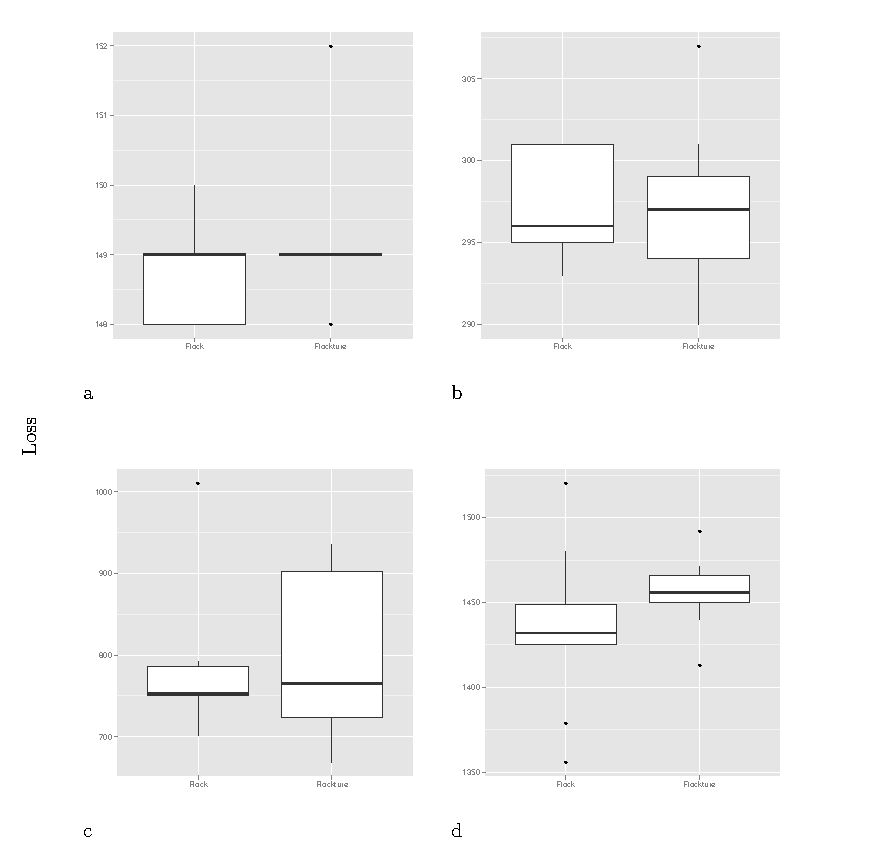
\includegraphics[width=.9\linewidth]{images/Figures-Pat/FlockvFlocktureLoss.pdf}
  \caption{Zero-one loss function for {\sc flock} and {\sc flockture} for 9 replicate 
  runs of simulated data sets comprised of five populations with varying
  levels of population differentiation:  $F_{ST} = $ (a) 0.03, (b) 0.02, (c) 0.01, and (d) 0.005.}
  \label{fig:FvFloss}
\end{center}
\end{figure}

{\sc flockure} ran much more quickly than {\sc flock}.  {\sc flock} 
averaged 1966.67 ($\pm 64.32$) seconds per run,
over all runs, while {\sc flockture} averaged 9.83 ($\pm 0.21$) seconds---a 200-fold improvement in 
speed. 

\subsection*{{\sc flockture} and {\sc structure}} 
As expected {\sc flockture} and {\sc structure} both perform extremely well on data sets with
well-differentiated populations. Infrequently, at higher levels of population differentiation the 
NA.NC and NA.C models in {\sc structure} exhibited large losses (Fig.~\ref{fig:uSatLoss})
resulting from the assignment of individuals from two groups into a single cluster while 
individuals from another group were separated into two clusters
with intermediate $q_i$ values (Fig.~\ref{fig:FvSdistruct} A). This phenomenon 
(only present in a single microsatellite data set) is an instance of {\sc structure}'s
Markov chain failing to converge well in the short runs we were using. As the subtlety of genetic structure 
increased, loss for both programs increased and differences in the performance of
each model with different marker types emerged.
For the microsatellite data set we observed that both programs
produce roughly equivalent results at higher levels of population differentiation. At intermediate 
values, the variance of the loss incurred by each model increased and certain models did marginally
better in assignment. No model did consistently better than others, until $F_{ST}$ dropped 
below 0.0136 after which the loss for {\sc flockture} was markedly larger as was the among-run
variance. The drastic increase in variance among runs was also observed with the SNP data sets. 
{\sc flockture} did, however, have consistently smaller loss than  {\sc structure} at high to intermediate 
values of $F_{ST}$. Once $F_{ST}$ fell below 0.016, however, {\sc structure} began correctly assigning a 
higher proportion of individuals. 

The number and length of plateaus {\sc flockture} encountered quickly %ref supp tables FLOCKTURE_PlateauTable_XX.pdf
diminished as the amount of differentiation among populations decreased (Supporting Information). For the microsatellite data sets,
when $F_{ST}$ was less than 0.0337, no plateau record
contained a plateau of length six or greater. No plateaus were observed 
(i.e. no two runs of {\sc flockture} gave exactly the same solution) when 
$F_{ST}$ was smaller than 0.02187. Results from the SNP data sets
were concordant.
Only simulated data sets with pairwise $F_{ST}$ values greater 0.0323 had plateau records with a 
plateau greater than six. Despite the lack of plateaus observed for many of the simulated data sets, 
graphs of the normalized likelihood values from the {\sc flockture} run with the highest 
likelihood were indicative of population structure (Fig~\ref{fig:FvSdistruct}).  

Plots of the normalized likelihood values from {\sc flockture} can be useful in discerning the presence of 
structure.  In situations where only a single run of {\sc flockture} produced a plateau of length 2 
(Fig.~\ref{fig:FvSdistruct} B) the variation in assignment of individuals among runs was qualitatively indistinguishable
and results were highly concordant with those of {\sc structure}. As population differentiation declines 
and plateaus are not observed, the run with the highest likelihood from {\sc flockture} still yields
clusters similar to those from {\sc structure} but with more variation among runs (Fig.~\ref{fig:FvSdistruct} C \& D).
As pairwise $F_{ST}$ decreases and the variation among {\sc flockture} runs increases, the normalized likelihood
values for assignment remain high in contrast to the $q_i$ values in each of the three models of {\sc structure}. 

  \begin{figure*}
\centering
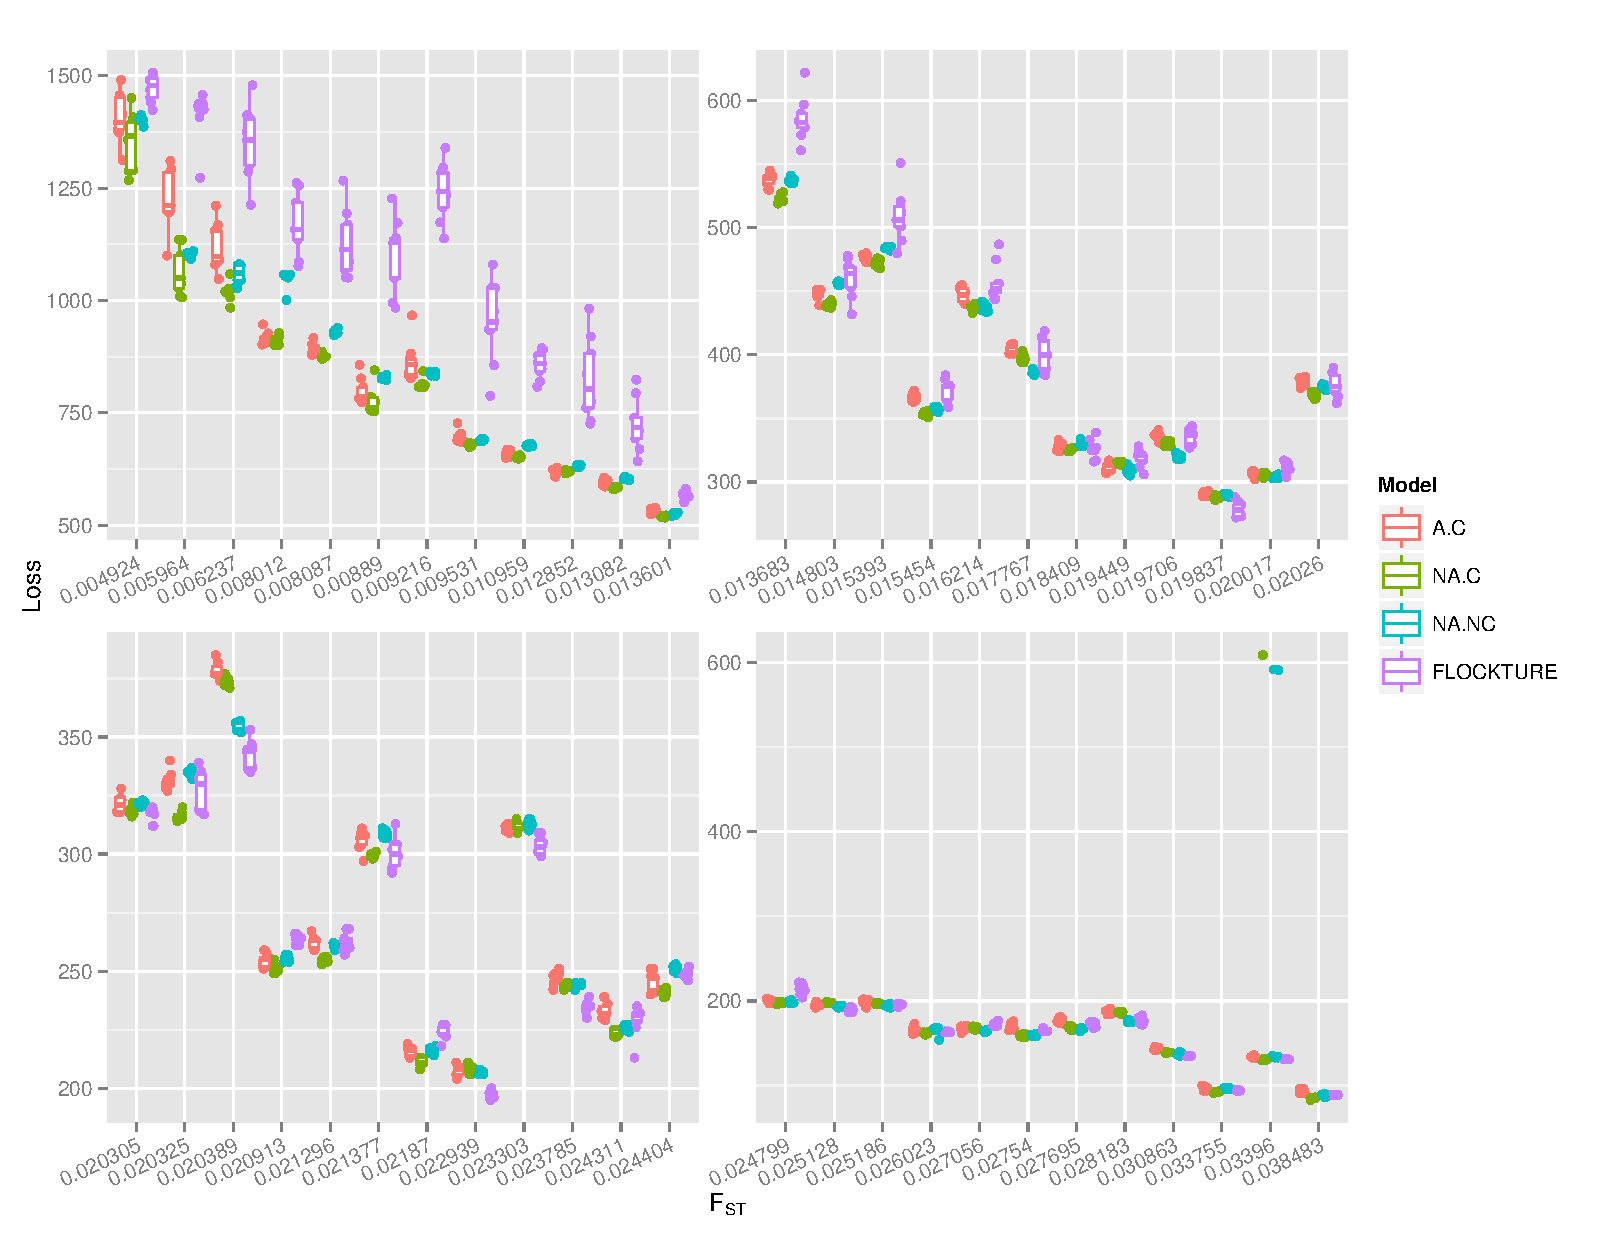
\includegraphics[width=.9\linewidth]{images/Figures-Pat/uSatLoss.pdf}%uSatloss_BW.pdf is a greyscale version
  \caption{Zero-one loss (lower values = better performance) for nine runs of {\sc flockture} and the admixture and correlated allele 
  frequency (A.C) model, the no-admixture and correlated allele frequency (NA.C) model, 
and the no-admixture and non-correlated allele frequency (NA.NC) model in {\sc structure}. Forty-eight 
data sets, composed of 2,000 individuals with 15 microsatellite genotypes comprising
5 populations of sizes 250, 250, 400, 550, and 550, were simulated to evaluate the performance
of both programs. }
  \label{fig:uSatLoss}
\end{figure*} 

 \begin{figure*}
\centering
  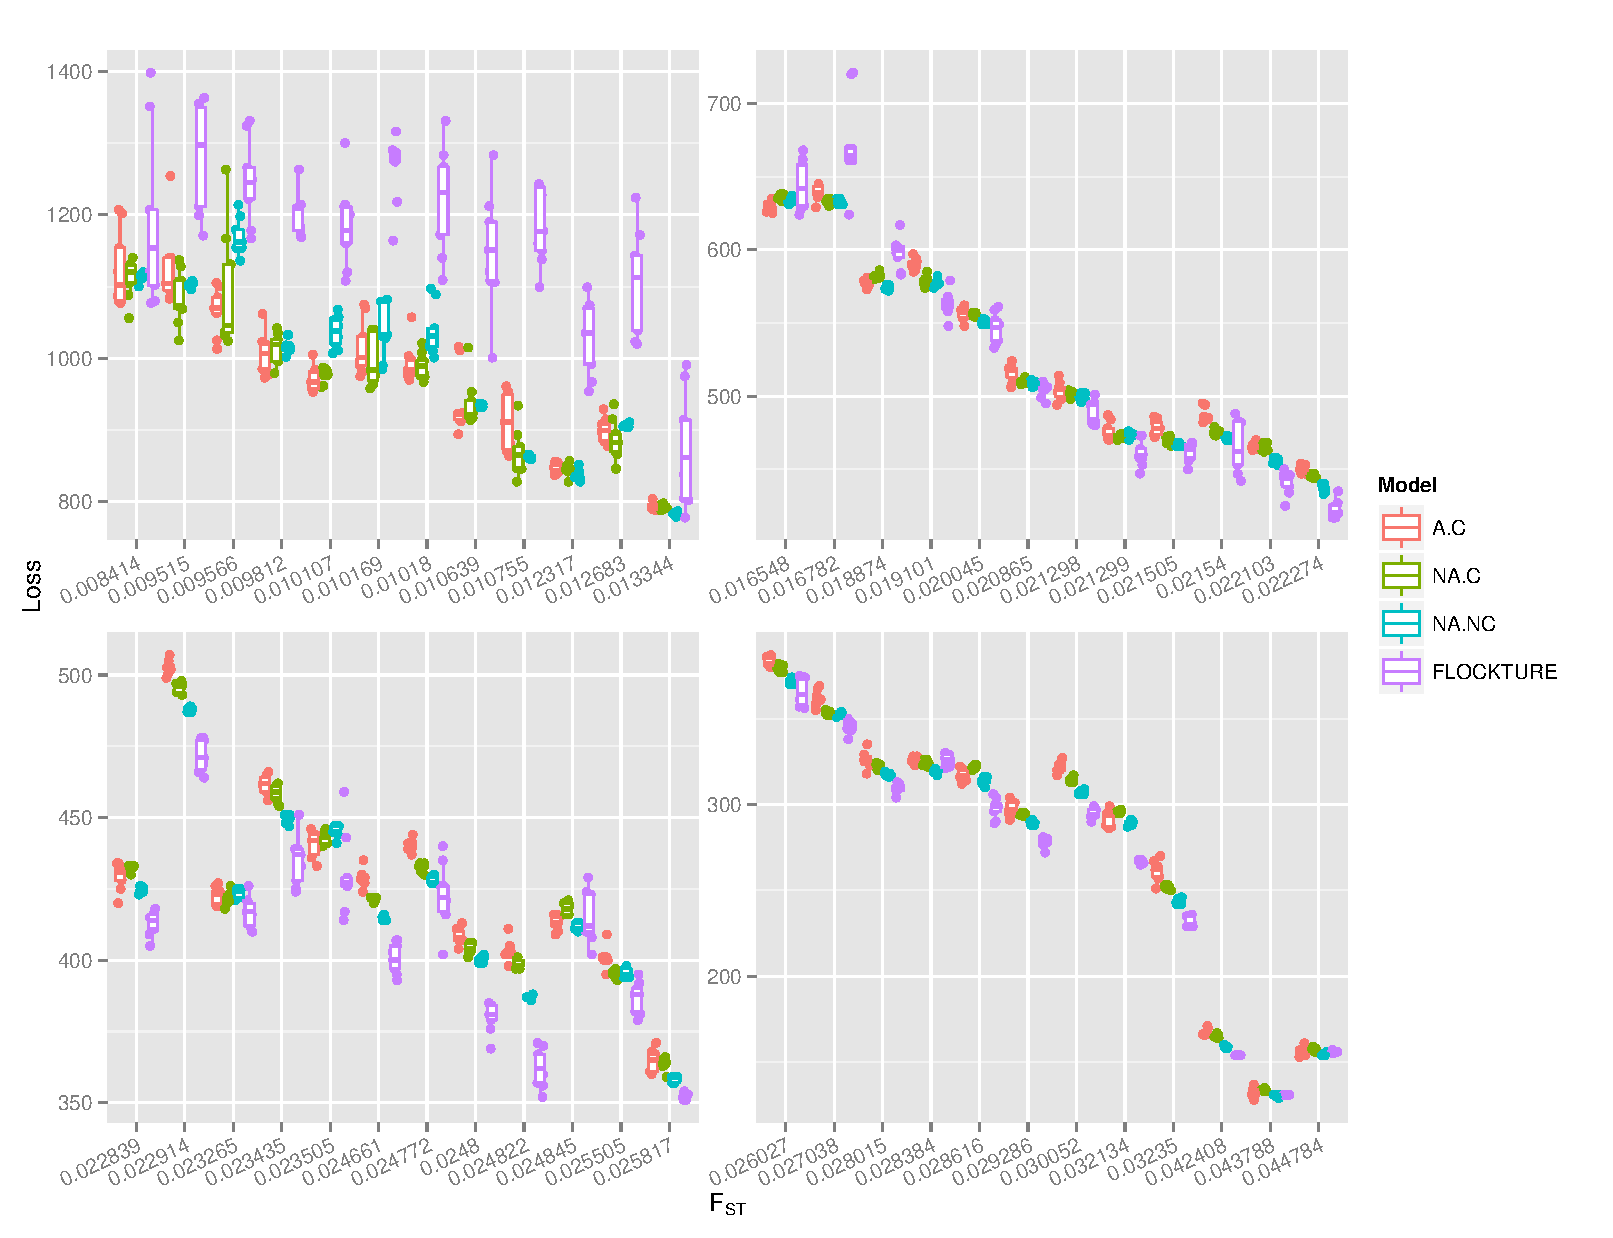
\includegraphics[width=.9\linewidth]{images/Figures-Pat/SNPloss.pdf}%SNPloss_BW.pdf is a greyscale version
  \caption{Zero-one loss for nine runs of {\sc flockture} and the admixture and correlated allele 
  frequency (A.C) model, the no-admixture and correlated allele frequency (NA.C) model, 
and the no-admixture and non-correlated allele frequency (NA.NC) model in {\sc structure}. Forty-eight 
data sets, composed of 2,000 individuals with 96 SNP genotypes comprising 
5 populations of sizes 250, 250, 400, 550, and 550, were simulated to evaluate the performance
of both programs. }
  \label{fig:SNPloss}
\end{figure*} 


 \begin{figure*}
\centering
  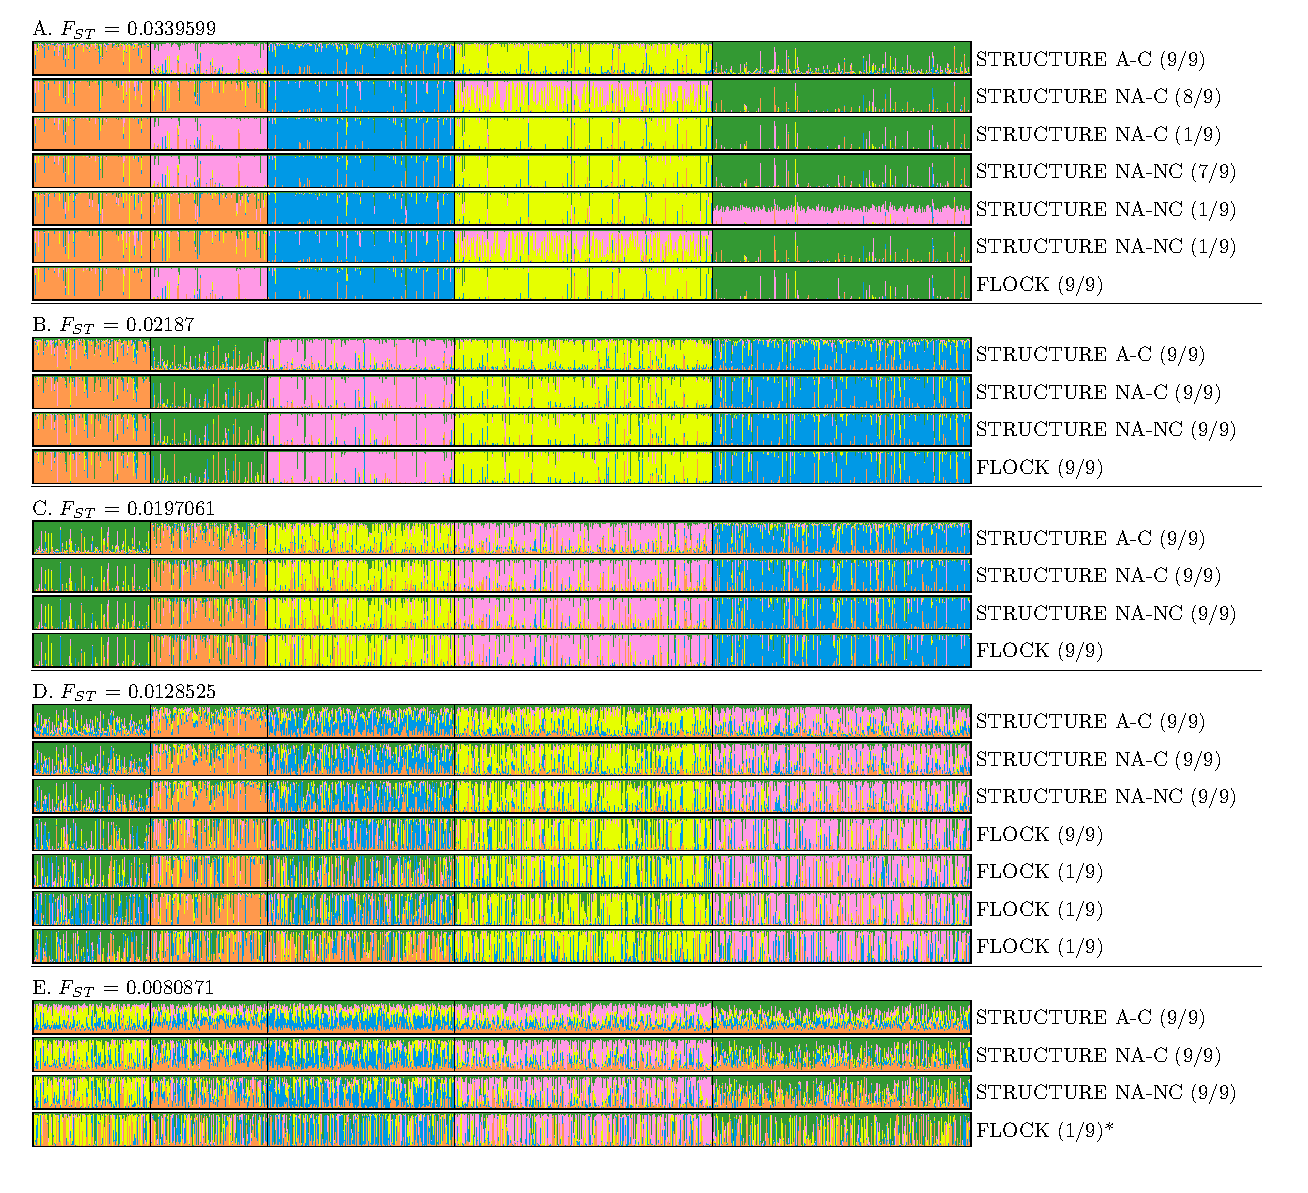
\includegraphics[width=.8\linewidth]{images/Figures-Pat/FlockturevStructureDistruct.pdf}%B+W version use 'FlockturevStructureDistruct_BW.jpg'
  \caption{
  Program {\sc distruct} plots of cluster membership probabilities of simulated individuals
  ($q_i$ values from {\sc structure} and the normalized likelihood values from {\sc flockture}). 
  Individuals are grouped left to right into their simulated population samples, and each 
  horizontal plot represents a run of the program
  {\sc structure}, or the ``longest-plateau-run'' from a series of runs in {\sc flockture} (unless
  there were no plateaus, in which case the run reaching the highest likelihood was chosen).
  Within horizontal plots, each individual is represented by a vertical bar composed of colored
  segments of lengths proportional to the various cluster membership probabilities.
  Each horizontal plot
  represents one of nine 
 runs of the programs  at $K$ = 5 (the true value of $K$). Three models were run in structure: the admixture and correlated allele 
  frequency (A.C) model, 
the no-admixture and correlated allele frequency (NA.C) model, 
and the no-admixture and non-correlated allele frequency (NA.NC) model. Numbers in 
parentheses following the model names give the number, out of 9, of replicate runs
that obtained the same visually-indistinguishable estimate. (Note that although many of {\sc flocktures}'s solutions in B--D were visually indistinguishable, they were not identical partitions, and would
hence be considered different for the purposes of creating a {\sc flock} plateau record.) In E, all 9
of {\sc flocktures}'s solutions were visually distinguishable, though we show only one.  Each simulation is comprised of
 five populations of sizes 250, 250, 400, 550, and 550 individuals with average pairwise $F_{ST}$ values
 indicated above each plot.}
  \label{fig:FvSdistruct}
\end{figure*}

\section*{Conclusions}
In the past decade, the use of genetic markers to identify population structure and to attempt inference of
the number of genetic clusters ($K$) in a collection has dramatically increased in the fields of ecology, evolution, 
epidemiology, and conservation
genetics. The most commonly used program for doing this is {\sc structure} \citep{Pritchardetal2000,Falushetal2003}, 
a full-featured program with many options that is widely-used, well-tested, and universally regarded as a standard tool amongst molecular ecologists. 


We have shown here that the model incorporated by {\sc flock} is analytically equivalent to {\sc structure}'s 
no-admixture model 
with non-correlated allele frequencies.
We adapted the source code of {\sc structure} to create {\sc flockture} and show that
{\sc flock} and {\sc flockture}  perform equivalently. 
In comparing results from {\sc flockture} and {\sc structure} 
on simulated data sets with varying levels of differentiation among populations
we find that the two programs give similar results.

Though we observed similar results
between the two programs at large values of $F_{ST}$, 
{\sc flockture}'s solutions consistently assigned fewer individuals correctly---and the
replicate solutions for individual data sets became more variable---at lower values of $F_{ST}$.
This is likely a consequence of the low population divergence which
makes it possible for many different allocations of individuals to
have roughly the same likelihood.
The likelihood surface defined on partitions of this space is then often
multimodal---possessing numerous local peaks and troughs.
The peak that the {\sc flock} algorithm finds is entirely determined by the initial, random, allocation of 
individuals, as the algorithm proceeds deterministically after the initial random allocation.
Decreasing $F_{ST}$ leads to more homogenous 
populations whose multilocus genotypes have a smaller difference in 
likelihood of assigning to any given cluster. This likely increases the number of
local peaks, leading {\sc flockture} and {\sc flock} to settle on different solutions in 
different runs. The problem presented by having multiple modes in the likelihood surface 
is not unique to {\sc flock}---{\sc structure} also can converge to 
different solutions in complex spaces; however our simulations suggest this is a more  
prevalent problem for the {\sc flock} algorithm.
{\sc flock} is not best-suited to species characterized by large
subpopulations and low divergence, as is the case with many 
marine fish.   
   

One of the advantages of {\sc flock} over other methods for genetic clustering
is reported to be the short processing time for each execution of {\sc flock}.
\citet{Duc&Tur2012} observed faster processing times relative to {\sc structure}.
Having implemented {\sc flockture} it is clear that the amount of computation required for a
single sweep of {\sc structure} is equivalent to an iteration of reallocation of individuals
in {\sc flock}.
Hence, if {\sc flock} and {\sc structure} took similar amounts of time for comparable
computations, one would expect that executing {\sc flock} once with 50 runs, each of 20 iterations,
would require about the same amount of time as running {\sc structure} on the same
data set for 1,000 sweeps.  Since it is recommended to run {\sc structure} longer than 1,000 sweeps, {\sc flock} should have a speed advantage. However, {\sc flock} requires far more 
time for each computation
than {\sc structure}, as is clear from the fact that it runs 200 times slower than 
{\sc flockture}.  Thus, for data sets comparable to the ones we simulated, one can expect
50 runs of 20 iterations in {\sc flock} (a standard execution of the program) to require as
much time as running {\sc structure} for 200,000 sweeps. This does not constitute
a speed advantage.
If {\sc flock} were to be implemented using good coding practices in a fast language,
rather than as a VBA routine in Microsoft Excel,
it could be made much faster. As it is, we found it preferable to implement our own version
of the {\sc flock} algorithm
in {\sc flockture} for our simulation assessment of the {\sc flock} algorithm.


Many researchers wish to estimate $K$, the number of subpopulations, from genetic data.  This is
a difficult task, statistically, because estimating $K$ is a problem in model selection, and hence can
be exquisitely sensitive to the priors on nuisance parameters as well as to departures from the underlying
model (e.g. clinal rather than demic structure). For these reasons, it seems inadvisable to us to
put too much stock in the inference of $K$ from any program, especially when population structure
is subtle. Accordingly, we have based our comparison of 
{\sc flockture} and {\sc structure} on their ability to correctly cluster individuals when the true value
of $K$ is known. 


While there has been lengthy 
discourse over the choice of estimators for $K$ in {\sc structure} 
\citep{Pritchardetal2000,Evannoetal2005,Wap&Gag2006,Gaoetal2011}, less has been written on how the number of 
individuals
and the number of starting allocations can affect not only the convergence of different runs of {\sc flock}, but also its 
inference of $K$. \citeauthor{Duc&Tur2012} developed estimation rules for $K$ based on simulated data 
sets with a modest number of individuals and different migration regimes and rates, numbers of loci, and $K$. 
By relying on the number of identical partitions obtained by {\sc flock} over multiple
runs as a means of supporting 
a particular $K$,  similar---but not identical---partitions
will provide no support to a given $K$. This could be problematic, 
since we have shown that even at intermediate
values of $F_{ST}$,  {\sc flockture} (and, by extension,
{\sc flock}) may converge to 
different cluster allocations in every run, so that no plateaus are encountered. 

The above presents a serious conundrum to the user of {\sc flock}.  On the one hand,
{\sc flock} clearly continues to provide useful inference about population structure
(as evidenced by the {\sc distruct} plots in Fig.~\ref{fig:FvSdistruct}), even when its
plateau record includes no plateaus; however, on the other hand, if there were no
plateaus for $K=5$ in our simulated data, then the {\sc flock} method would lead to an estimate of $K$ that
was either "undecided" or some value less than $K$ as the lower bound or point estimate of $K$. The authors of {\sc flock}
discourage users from making any inference at a value of $K$ that is not
the value estimated by {\sc flock}, because, ``outside the estimated $K$, no partitions from {\sc flock}
 should be considered. Therefore\ldots clusterings from {\sc flock}\ldots for all $K$ except the estimated one are just
 irrelevant and not valid''(Pierre Duchesne, pers. comm).  To be specific, following 
this advice of {\sc flock}'s authors would have led to discarding {\sc flockture}'s
results for any $F_\mathrm{ST} < 0.032$ (almost 90\% of our simulated data sets); even those that are
manifestly quite accurate---some competitive
with or even superior to {\sc structure}'s estimate.  We surmise that this problem with the guidance on 
{\sc flock} stems from the fact that the {\em ad-hoc} rules developed by
\citeauthor{Duc&Tur2012} for estimating $K$ with {\sc flock} were developed empirically
by reference to a small set of simulations over a fairly limited range of sample sizes.  Since our simulated
samples (made to mimic the sorts of large, real data sets we collect in our labs)
fall outside the range of values explored
by \citeauthor{Duc&Tur2012}, it appears that {\sc flock}'s rules of use are inappropriate, 
and perhaps over-restrictive for these data sets.  Researchers with data that similarly fall beyond the range of 
data sets tested in \citet{Duc&Tur2012} may wish to approach {\sc flock} analysis with
caution, or may choose to rely on other programs.


 
Often, newly-developed algorithms come to be understood within more general contexts and 
frameworks, and this, in turn, can help guide improvement of those algorithms.  For example, in population
genetics, the ``Markov recursion'' algorithm of \citet{Gri&Tav1994-AI} was identified by \citet{Felsensteinetal1999} 
as a special case of importance sampling \citep{Ham&Han1964}, a perspective which allowed 
\citet{Ste&Don2000} to improve upon the algorithm dramatically.  Here we have identified the {\sc flock}
algorithm as a limiting case of simulating annealing upon {\sc structure}'s no-admixture model with uncorrelated
allele frequencies. We hope this will
help users to understand and interpret {\sc flock}'s behavior and will provide insights that may be useful 
in the potential development of {\sc flock} or other clustering algorithms.   


\section*{Acknowledgments}
We are grateful to Kristen Ruegg and Robin Waples for helpful comments on a draft of this paper.
Comments and suggestions from an anonymous referee and Pierre Duchesne helped to strengthen the
paper considerably.
P. Barry was supported by a fellowship from the Rasmuson Foundation.